\cbcomment{This is copied from Jiajia's paper for now, and the graphics are in there as placeholders}
This section provides some essential formal background on tensors. Several of the examples and definitions are taken from the excellent overview by Kolda and Bader~\cite{Kolda:2009}.

A tensor can be interpreted as a multi-way array, as illustrated graphically in \reffig{fig:3dtensor}. This is a 3rd-order tensor. 
We represent tensors by bold underlined capital letter, e.g., $\T{X} \in \R^{I \times J \times K}$. 
The \emph{order} of a tensor is the number of its dimensions or modes, which in the example is 3.
Matrices and vectors are special cases of tensors.
Matrices are 2nd-order tensors, and we denote them by boldface capital letters, e.g., $\M{A} \in \R^{I \times J}$.
Vectors are 1st-order tensors, and we denote them by boldface lowercase letters, e.g., \V{x}.
The elements of a tensor are scalars, and we denote them by lowercase letters, such as $x_{ijk}$ for the $(i,j,k)$ element of a 3rd-order tensor \T{X}.

Given a tensor, we can also ask for a variety of \emph{sub-tensors}.
One form of sub-tensor is a \emph{slice}, which is a 2-dimensional cross-section of a tensor.
\RefFigure{fig:tensor-example}(a) illustrates the concept of slices, showing different slices of a 3rd-order tensor.
Another form of sub-tensor is a \emph{fiber}, illustrated in \reffig{fig:tensor-example}(b).
A fiber is a vector extracted from the tensor, and is defined by fixing every index by one~\cite{Kolda:2009}.

Since slices are all matrices, they can for the 3rd-order example of \reffig{fig:tensor-example}(a) be represented by $\M{X}_{i::}$, $\M{X}_{:j:}$, and $\M{X}_{::k}$.
%For instance, the columns of the matrix $\mathbf{A}=[\mathbf{a_1}, \mathbf{a_2}, \dots, \mathbf{a_J}] \in \R^{I \times J}$ are denoted by $\mathbf{a_j}$. 
In this paper, we consider double-precision real-valued elements for all tensors, matrices, and scalars.

\RefFigure{fig:tensor-example}(b) gives three fibers of the tensor, denoted by $\V{x}_{:jk}, \V{x}_{i:k}, \V{x}_{ij:}$.

\begin{figure}
  \centering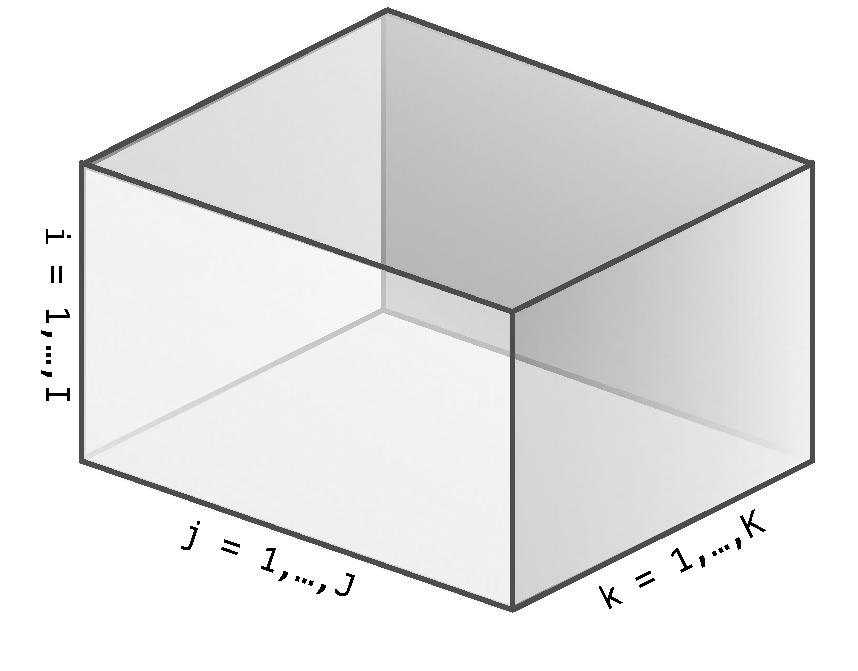
\includegraphics[width=0.4\linewidth]{figs/3dtensor}
  \caption{Example of a 3d tensor.}
  \label{fig:3dtensor}
\end{figure}

\begin{figure}[htbp]
    \centering
    \begin{tabular}{>{\centering\arraybackslash}p{0.45\textwidth}}
%    \includegraphics[scale=0.15]{figs/tensor-example} \\
%    (a) A third-order tensor $\T{X} \in \R^{I \times J \times K}$ (TODO: redo) \\\\
    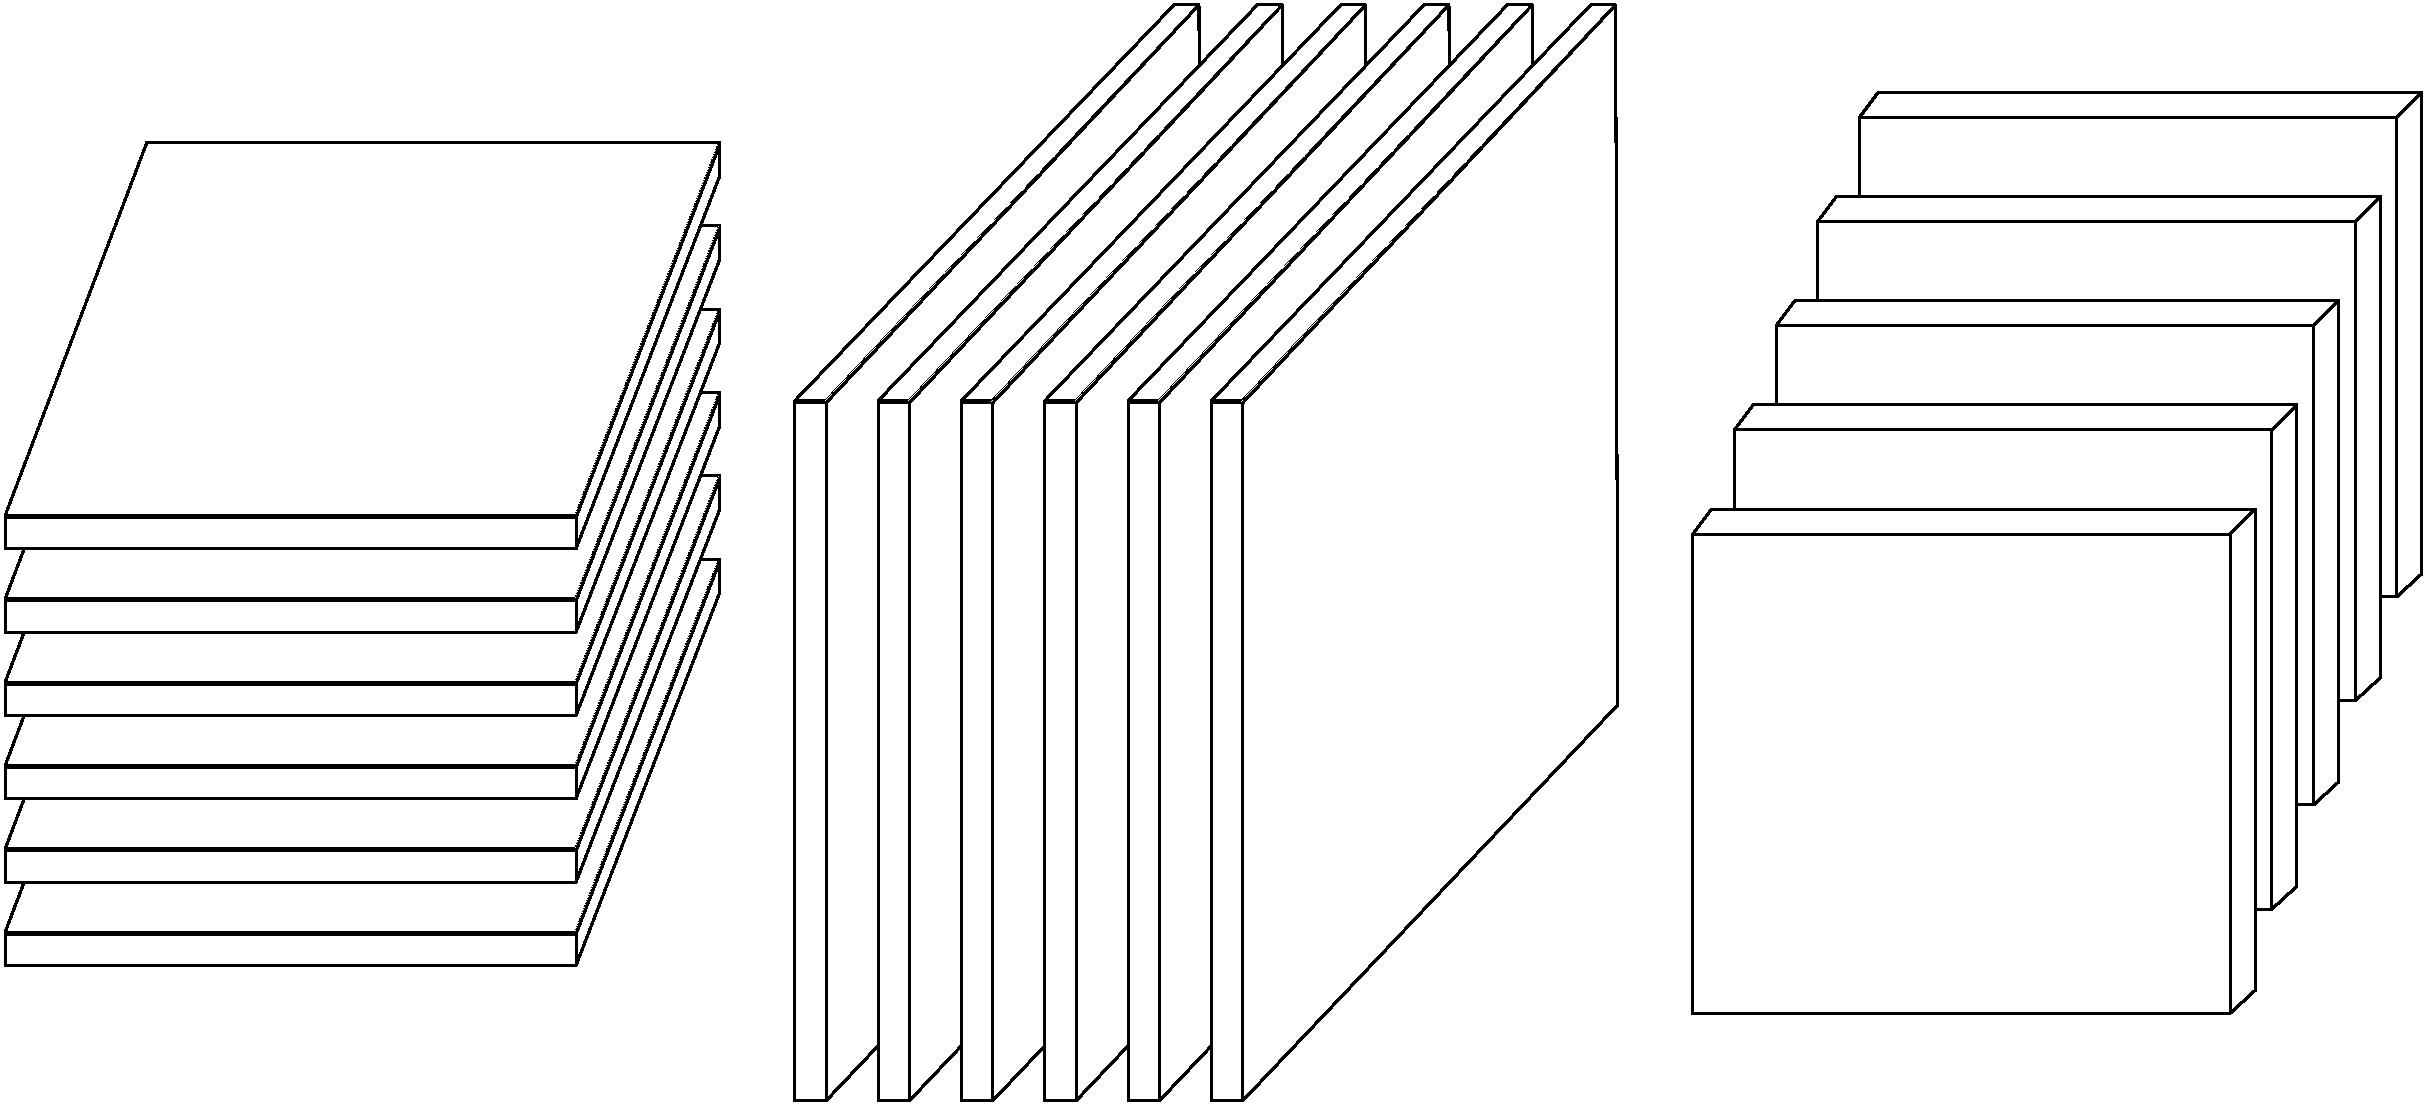
\includegraphics[width=0.55\linewidth]{figs/slices_own} \\
    (a) Horizontal, lateral and frontal slices of a third order tensor \\\\
    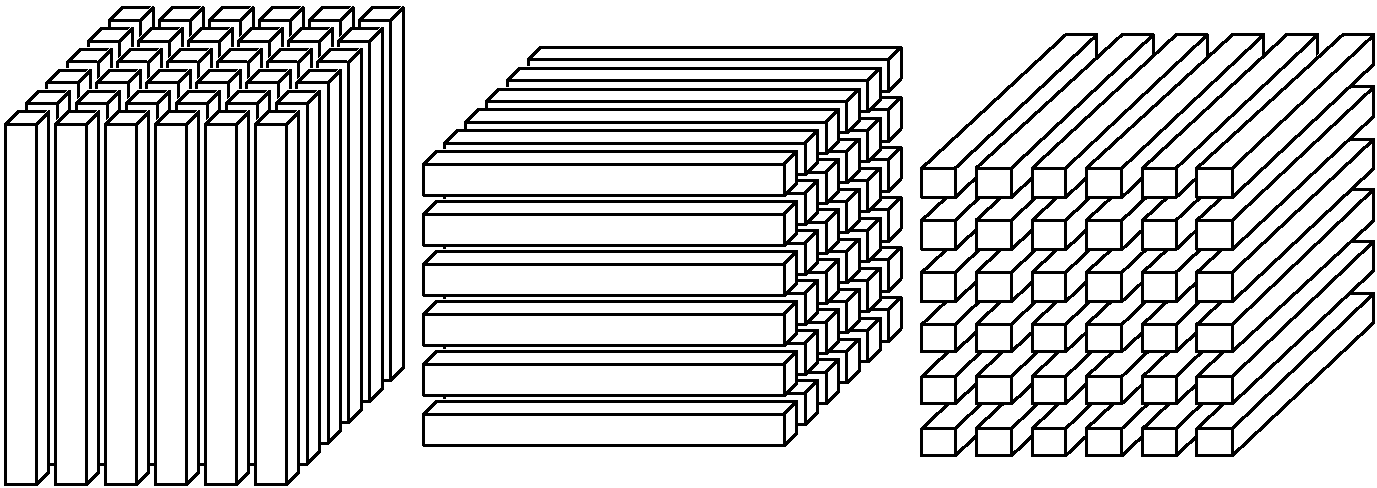
\includegraphics[scale=0.2]{figs/fibers_own} \\
    (b) Column (mode-1), row (mode- 2), and tube (mode-3) fibers of a third order tensor. \\
    \end{tabular}
    \caption{Some sub-tensor views of the third-order tensor $\T{X} \in \R^{I \times J \times K}$.}
    \label{fig:tensor-example}
\end{figure}

Examples of tensor operations include the mode-$n$ product introduced in \refsec{sec:intro}, tensor contraction, and Kronecker product~\cite{Kolda:2009}.
Since the mode-$n$ product is among the most widely used of these primitives, we focus on it in this paper and refer to it alternately as the \acf{Ttm}, following the terminology of the \TensorToolbox~\cite{TTB_Software}.
%Thus, we focus on mode product as our primary example of tensor multiplications in this paper.
Comprehensive surveys of other tensor operations appear elsewhere~\cite{Kolda:2009,CICHOCKI:2014}.

The \TTM between a tensor $\T{X} \in \R^{I_1 \times I_2 \times \cdots \times I_N}$ and a matrix $\M{U} \in \R^{J \times I_n}$ is another tensor $\T{Y} = \T{X} \times_n \M{U}$, where $\T{Y} \in \R^{I_1 \times \dots \times I_{n-1} \times J \times I_{n+1} \times \cdots \times I_N}$.
One way to precisely define \TTM is to express it as the element-wise computation,
\begin{eqnarray}
  y_{i_1 \dots i_{n-1} j i_{n+1} \dots i_N}
    & = & (\T{X} \times_n U)_{i_1 \dots i_{n-1} j i_{n+1} \dots i_N} \nonumber \\
    & = & \sum_{i_n=1}^{I_n} x_{i_1 i_2 \dots i_N} u_{ji_n}.
  \label{eq:moden-ele}
\end{eqnarray}
Note that where the input tensor \T{X} is of length $I_n$ in its \varTh{n} mode, the result \T{Y} is of length $J$ in its \varTh{n} mode.
Typically, $J$ will be much less than $I_n$, which we show has important consequences for performance in \refsec{sec:obser}.


The traditional way to execute a \TTM is through \emph{matricization}, also called \emph{unfolding} or \emph{flattening} in the literature.
That is, \TTM is equivalent to a matrix-matrix multiplication in the form,
%
\begin{equation}\label{eq:moden-mat}
  \T{Y} = \T{X} \times_n U \Leftrightarrow \M{Y}_{(n)} = \M{U} \M{X}_{(n)},
\end{equation}
%
where $\M{Y}_{(n)}$ and $\M{X}_{(n)}$ denote the matricized forms of $\T{Y}$ and $\T{X}$, respectively.
For a mode-$n$ product, matricization logically reorders the elements of an order-$N$ tensor into a matrix by exchanging mode $n$ and the leading mode.
The leading mode is dictated by data layout. If data is located in row-major, the last dimension (mode-$N$) is the leading mode.
For instance, a $3 \times 4 \times 2$ tensor with elements from $1$ to $24$ can be arranged as a $3 \times 8$ matrix, or a $4 \times 6$ matrix, or a $2 \times 12$ matrix.
In the tensor context, \emph{vectorization}, $\V{y} = \makeVec(\T{X})$, refers to converting a tensor into an equivalent vector.
The reverse process of creating a tensor from a matrix or vector is called \emph{tensorization}.

\begin{equation}
\label{eq:moden-matricization}
\begin{split}
\M{X}_{(1)} = \left[
\begin{array}{cccccccc}
1 & 4 & 7 & 10 & 13 & 16 & 19 & 22 \\
2 & 5 & 8 & 11 & 14 & 17 & 20 & 23 \\
3 & 6 & 9 & 12 & 15 & 18 & 21 & 24 
\end{array}
\right],\\
\M{X}_{(2)} = \left[
\begin{array}{cccccc}
1 & 2 & 3 & 13 & 14 & 15 \\
4 & 5 & 6 & 16 & 17 & 18 \\
7 & 8 & 9 & 19 & 20 & 21 \\
10 & 11 & 12 & 22 & 23 & 24 
\end{array}
\right],\\
\M{X}_{(3)} = \left[
\begin{array}{ccccccc}
1 & 2 & 3 & \dots & 10 & 11 & 12 \\
13 & 14 & 15 & \dots & 22 & 23 & 24
\end{array}
\right].
\end{split}
\end{equation}

\subsubsection{Multilinear Rank}
Computing rank is NP complete~\cite{HastadRanknp}, and best-rank approximation is ill-posed~\cite{Kolda09tensordecompositions}
\subsubsection{Tensor Algebra}

\subsubsection{Tensor Contractions}

\subsubsection{Tensor Network Diagrams}
\begin{figure}
  \centering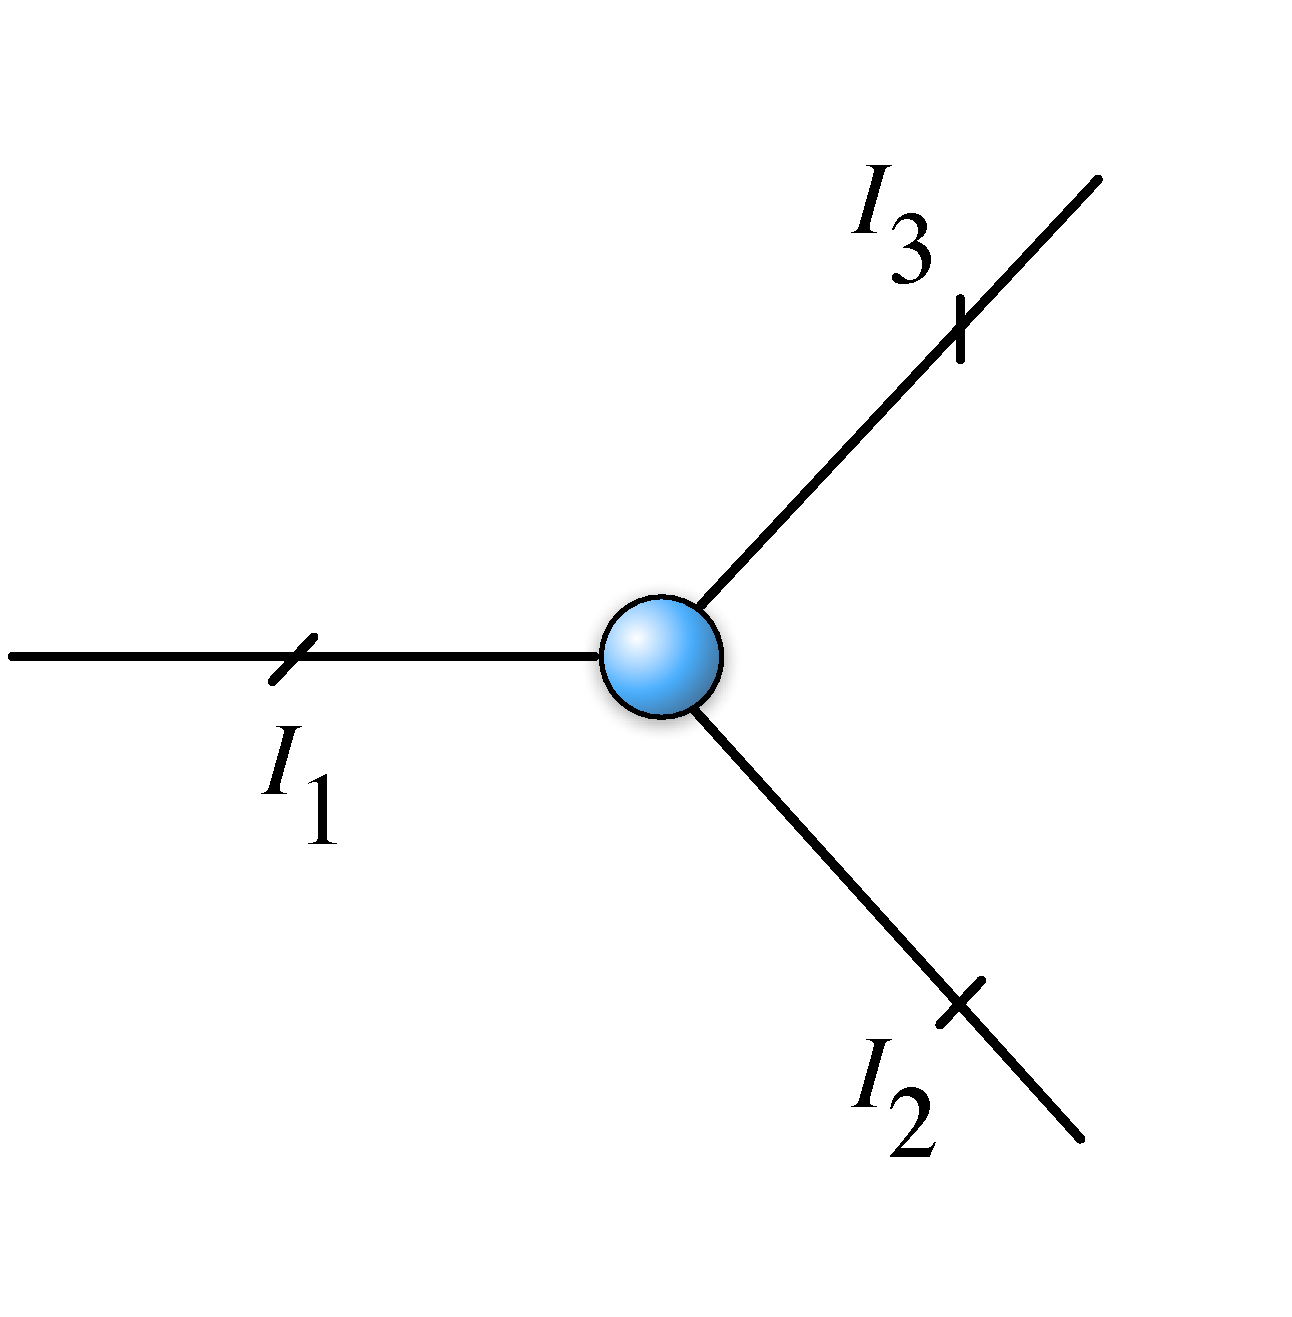
\includegraphics[width=0.3\linewidth]{figs/3dtensornet}
  \caption{Example of 3d tensor representation as a tensor network.}
  \label{fig:3dtensornet}
\end{figure}
% eof
